\documentclass[letterpaper,12pt]{article}

%\setlength{\parindent}{0in}
%\usepackage{fullpage} 
\usepackage{amsmath}
\usepackage{amssymb}
\usepackage{enumerate}
\usepackage{graphicx}
\usepackage[table]{xcolor}
\usepackage{dcolumn}
\usepackage[english]{babel}
\usepackage{setspace}
%\singlespacing
\onehalfspacing
%\doublespacing
%\setstretch{1.1}
\oddsidemargin 0.0in
\textwidth 6.5in
\newcolumntype{.}{D{.}{.}{-1}}
\newcommand*{\myalign}[2]{\multicolumn{1}{#1}{#2}}
% Alter some LaTeX defaults for better treatment of figures:
% See p.105 of "TeX Unbound" for suggested values.
% See pp. 199-200 of Lamport's "LaTeX" book for details.
%   General parameters, for ALL pages:
\renewcommand{\topfraction}{0.9}	% max fraction of floats at top
\renewcommand{\bottomfraction}{0.8}	% max fraction of floats at bottom
%   Parameters for TEXT pages (not float pages):
\setcounter{topnumber}{2}
\setcounter{bottomnumber}{2}
\setcounter{totalnumber}{4}     % 2 may work better
\setcounter{dbltopnumber}{2}    % for 2-column pages
\renewcommand{\dbltopfraction}{0.9}	% fit big float above 2-col. text
\renewcommand{\textfraction}{0.07}	% allow minimal text w. figs
%   Parameters for FLOAT pages (not text pages):
\renewcommand{\floatpagefraction}{0.7}	% require fuller float pages
% N.B.: floatpagefraction MUST be less than topfraction !!
\renewcommand{\dblfloatpagefraction}{0.7}	% require fuller float pages


%REQUIREMENTS:
% 1.  Determine what metrics are appropriate for this situation.  Use them for all subsequent requirements. 
%
% 2.  Without considering sequencing or ranges, do a �back-of-the-envelope� simulation using Excel to model the number of hits per ExWar ship based on a salvo of 150 Intracets, and whether or not the ExWar ships are sunk.  This should be similar to the example worked in class. Make 500 runs and report statistics on as many of your metrics as possible. Support your back of the envelope calculation with a simple range-target graph. (Big Hint: there is an Excel demo, which we will discuss in class in detail, in the course materials folder for module 7 that steps you through this.) 
%
% 3.  Model the defense of the 4 ExWar ship force against the incoming swarm of missiles, including sequencing and ranges.  Describe how you will (or will not) account for the geometry and dispersion of your ship formation.
%
% 4.  Implement your model in Extend.  Organize, label, and document your file.
%
%5.  Based on 500 runs of your Extend model, estimate the average, best, and worst outcomes of your metrics resulting from a salvo of 150 Intracets fired to have simultaneous arrival in the vicinity of the ships.
%
% 6.  For the given force package, determine a cost-effective set of  improvements to either the sensors,  standard missile,  EW countermeasures, or the CIWS that results in 90% confidence of a less than a 1% chance of losing an ExWar ship from a salvo of 150 Intracets fired to have simultaneous arrival in the vicinity of the ships.  Make plausible assumptions about what your changes will cost. Use a designed experiment or optimization search to explore your trade space, and document why you chose that particular approach and its particulars. 
%
% 7.  Without changing the combat systems from the initial configuration, determine the number of cruisers or destroyers necessary to result in a less than 1% chance of losing an ExWar ship from a salvo of 150 Intracets fired to have simultaneous arrival in the vicinity of the ships.  Again, assume no changes to the original capabilities. Make an assumption about what your changes will cost.
%
% 8. Construct a cost �effectiveness curve for your answers to (6) and (7).
%
% 9.  If you wanted to examine the scenario space (i.e. the spanning set of stressing scenarios), how do you think the results of your analysis would change for a) 50 incoming missiles, or b) 200 incoming missiles?  You do not need to redo the analysis in detail, but support your assertion with at least a trial run or BOE analysis.
%
% 10.  What is the effect if the Intracets are not fired to impact simultaneously, but instead have a common expected arrival time with a standard deviation of 30 seconds?  What is the effect if the first 25% of the missiles are targeted against the cruisers and destroyers, not governed by RCS?
%
% 11. 
% a) Summarize your results in a concise, well-written, and well-illustrated report.  Document your Extend model.  Use spreadsheets or an Extend database for your input and output.  Your well-written, well-illustrated report is due at the eleventh, and last, class meeting. 
%
% b) Include a summary brief as an appendix (no more than 12 slides).  During our last class meeting, each team will be asked to discuss their results using their summary brief.  Ensure that your team members� names are included in all file names.  Recall that you must use new partners for this project.


\title{Project 3 \\ Group 4}
\author{Douglas Brown \\ Jessica Hale \\ Steve Mazza \\ Daniel Torres}
\date{March 21, 2012}

\begin{document}
\maketitle
\tableofcontents
\listoffigures
\listoftables
\pagebreak

\section{The Problem}
Through modeling and simulation we address the problem of defending high value targets against a salvo of one-hundred, fifty Intracets against a US Naval fleet of 2 Cruisers, 3 Destroyers, and 4 Expeditionary Warships (ExWars).  What we find is that with the given number of Intracets, the fleet is quickly overwhelmed and cannot adequately contend with the incoming strike.

The parameters we are given are as follows and illustrated in Figure \ref{fig:ov1} on page \pageref{fig:ov1}.  The Intracets are launched from a range of 100,000 yards and have a 59 second travel time to their maximum engagement range at 80,000 yards.  This is followed by a 166 second travel time before they reach the maximum detection range at 24,000 yards.  This initiates a critical window of 59 seconds after which the Intracets are inside of our minimum engagement range of 4,000 yards.  Inside this range, ship defense is relegated to the close-in weapon systems.

\begin{figure}[h!tbp]
	\begin{center}
		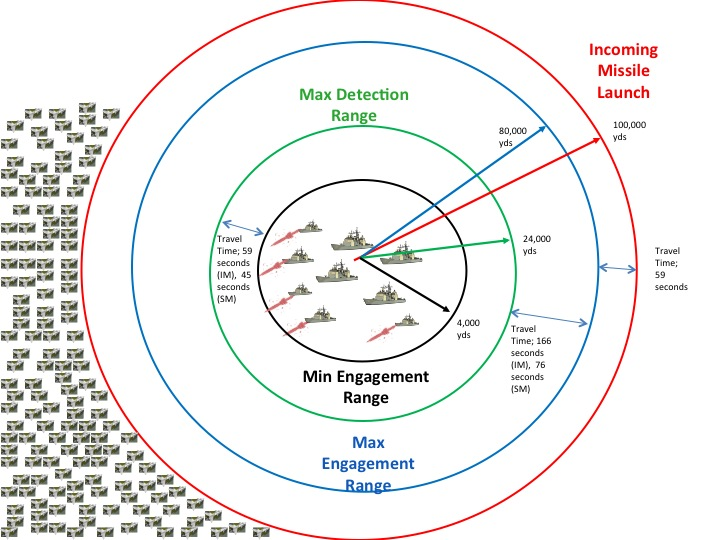
\includegraphics[scale=0.45]{images/info-graphic.jpg}
	\end{center}
	\caption{High level problem description.}
	\label{fig:ov1}
\end{figure}

% Requirement 1-3
\begin{samepage}
We use back of the envelope (BOE) calculations and ExtendSim modeling to investigate the effectiveness of ship-to-air missile and close-in weapon system (CIWS) defenses against Intracets fired, \emph{en masse}, against a small fleet of Destroyers, Cruisers, and ExWars.  During the modeling, we capture the following metrics that we use to assess the effectiveness of these defenses.  These are summarized in Table \ref{tab:metrics} below.

\begin{table}[h!tbp]
	\begin{center}
		\begin{tabular}{ll}
			\hline
			\myalign{c}{\textbf{Type}} & \myalign{c}{\textbf{Metric}} \\
			\hline\hline
			Hits	& \\
			& ExWar Hits \\
			& Cruiser Hits \\
			& Destroyer Hits \\
			Sinks & \\
			& ExWars Sunk \\
			& Cruisers Sunk \\
			& Destroyers Sunk \\
			Intracets Killed & \\
			& Killed by S2 \\
			& Killed by CIWS \\
			\hline
		\end{tabular}
	\end{center}
	\caption{Metrics captured during modeling and simulation}
	\label{tab:metrics}
\end{table}
\end{samepage}

These metrics were chosen based on their influence and impact on several key factors which weighed most heavily in our analysis.  Reducing the potential for loss of life is the single largest factor for us as Sailors and Warfighters form the basis of our national defense.  Secondary high value assets principally include ships as the cost to replace or repair damaged or sunk ships is measured in the billions of dollars.  This damage or loss also results in the loss or reduction of overall fleet capability and speaks to our national defense and wartime readiness.  The time required for replacement or repair is substantial and measured in months, if not years.  Lastly, we were concerned with measurement of the effectiveness of ship defense systems.

\section{Modeling}
\begin{samepage}
We begin with BOE calculations using Microsoft Excel, setting up four (4) ExWars, two (2) Cruisers, and three (3) Destroyers.  
The calculations take into account 150 simultaneously fired Intracets. Range Target analysis was conducted to determine only 85 S2 missile launches were possible within the firing window to intercept the Intracets.  This time based firing limitation was integrated into the BOE calculations. The analysis of 500 simulated runs is summarized in Table \ref{tab:BOESummary} on page \pageref{tab:BOESummary} and in the  Range Target graph  shown in Figure \ref{fig:rangeTarget} on page \pageref{fig:rangeTarget}.

\begin{table}[h!tbp]
	\begin{center}
		\begin{tabular}{l.}
			\hline
			\myalign{c}{\textbf{Metric}} & \myalign{c}{\textbf{Value}} \\
			\hline\hline
			\multicolumn{2}{c}{\textbf{Average Ships Sunk}} \\
			ExWar & 3.310 \\
			Cruiser & 0.478 \\
			Destroyer & 0.578 \\
			\multicolumn{2}{c}{\textbf{Average Ship Hits}} \\
			ExWar & 49.342 \\
			Cruiser & 1.702 \\
			Destroyer & 1.000 \\
			\multicolumn{2}{c}{\textbf{Average Intracets Killed}} \\
			SM Kills & 64.520 \\
			ExWar CIWS Kills & 8.446 \\
			Cruiser CIWS Kills & 1.164 \\
			Destroyer CIWS Kills & 0.814 \\
			\hline
		\end{tabular}
	\end{center}
	\caption{Summary of metrics from BOE calculations (500 runs)}
	\label{tab:BOESummary}
\end{table}
\end{samepage}

% Requirement 4
For further investigation and understanding, we implement our model in ExtendSim.  This allows a finer granularity as we are able to see the effects of the simulation at any point in time for a given iteration.  In order to focus on the effects of the Intracets we simplify our model with regard to geometry and dispersion by assuming a single point that the fleet occupies.  Within that point we still account for radar cross section and the numbers of various types of ships.

\subsection{ExtendSim Model}
A breakdown of our ExtendSim model is presented and discussed in order to provide better clarity in how we performed our simulation.

\begin{samepage}
\begin{figure}[h!tbp]
	\begin{center}
		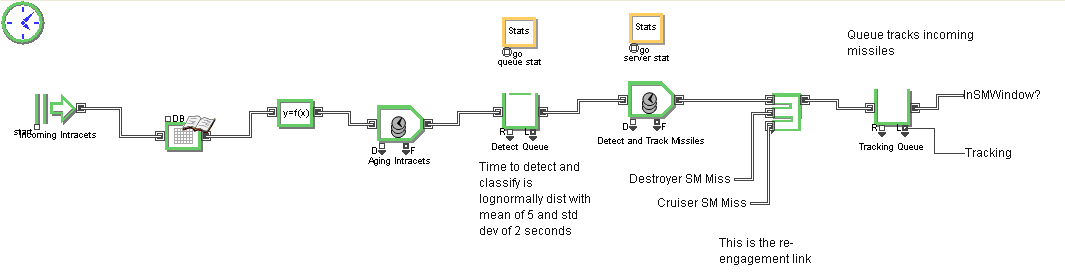
\includegraphics[scale=0.35]{images/0-Queues.png}
	\end{center}
	\caption{Initial queues.}
	\label{fig:queues}
\end{figure}

In Figure \ref{fig:queues} on page \pageref{fig:queues} the 150 Intracets are generated in the system and aged for the duration of their inbound flight until they enter the Detect and Track queue.  It is in this leg of the simulation where Destroyers and Cruisers can potentially re-acquire a missed Intracet, time allowing.  For surface-to-air missile defense, the Tracking queue represents the critical window of opportunity.
\end{samepage}

\begin{samepage}
\begin{figure}[h!tbp]
	\begin{center}
		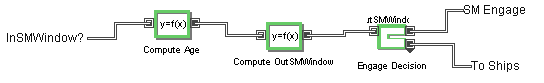
\includegraphics[scale=0.5]{images/1-Aging.png}
	\end{center}
	\caption{Determine aging of Intracets after they are picked up.}
	\label{fig:aging}
\end{figure}
The crucial calculation is performed as shown in Figure \ref{fig:aging} on page \pageref{fig:aging} to see if the Intracets remain in the window of opportunity for the surface-to-air missiles, beyond which they must be handled by the far less capable close-in weapon system.
\end{samepage}

\begin{samepage}
\begin{figure}[h!tbp]
	\begin{center}
		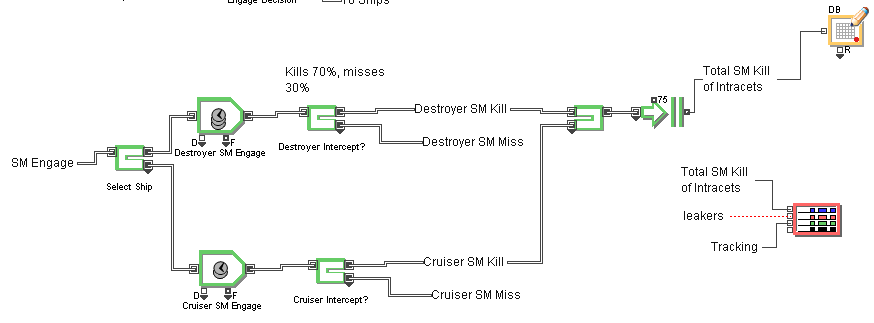
\includegraphics[scale=0.5]{images/2-InitialKills.png}
	\end{center}
	\caption{Intracets killed by surface-to-air missiles.}
	\label{fig:initialkills}
\end{figure}
Having acquired their targets, the surface-to-air missiles are used to the best advantage of the fleet to neutralize the Intracets (see Figure \ref{fig:initialkills} on page \pageref{fig:initialkills}).  An initial determination is made as to the available ship (Destroyer or Cruiser) and then a calculation is made to calculate hits and misses.  Lastly, kills are recorded, leakers are logged, and the misses are passed through to the close-in weapon systems.
\end{samepage}

\begin{samepage}
\begin{figure}[h!tbp]
	\begin{center}
		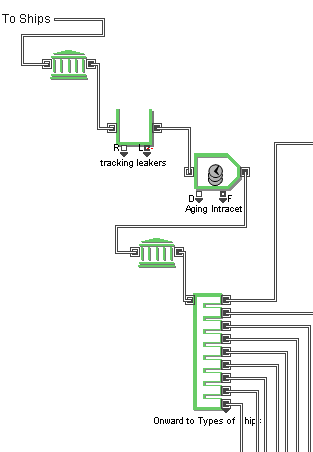
\includegraphics[scale=0.4]{images/3-Leakers.png}
	\end{center}
	\caption{Distribute leakers to fleet by radar cross section.}
	\label{fig:leakers}
\end{figure}
All remaining Intracets are entered into a queue and aged appropriately (see Figure \ref{fig:leakers} on page \pageref{fig:leakers}).  During this time they are \emph{assigned} to a remaining ship based on radar cross section and number.
\end{samepage}

\begin{samepage}
\begin{figure}[h!tbp]
	\begin{center}
		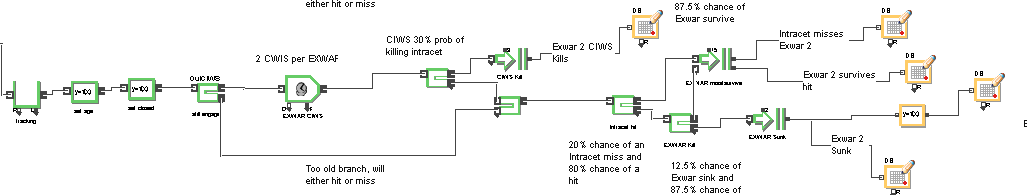
\includegraphics[scale=0.4]{images/4-CIWS.png}
	\end{center}
	\caption{Model of the close-in weapon system.}
	\label{fig:ciws}
\end{figure}
During the remaining aging of the Intracets the close-in weapon systems attempt to neutralize as many as possible.  In Figure \ref{fig:ciws} on page \pageref{fig:ciws} each ship's CIWS picks up missiles from the queue.  Acquisition time and aging are the critical calculations as time is in short supply.  For those Intracets remaining, a calculation is made to determine both effectiveness (Did they hit their target?) and lethality (Did their target survive the hit?)  All relevant metrics are captured in the database.
\end{samepage}

\begin{samepage}
\begin{figure}[h!tbp]
	\begin{center}
		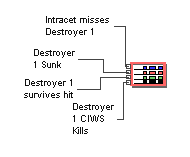
\includegraphics[scale=0.7]{images/5-Reporting.png}
	\end{center}
	\caption{Collection of selected metrics.}
	\label{fig:reporting}
\end{figure}
Lastly, Figure \ref{fig:reporting} on page \pageref{fig:reporting} some final metrics are captured and reported for the discrete simulation.
\end{samepage}

\subsection{Model Results}
% Requirement 5
We exercise our ExtendSim model by performing five hundred runs and calculate the average, best, and worst outcomes resulting from a salvo of one-hundred, fifty Intracets with simultaneous arrival time at our fleet.  Our calculated results are summarized in Tables \ref{tab:missileKillMetrics} - \ref{tab:shipsHitMetrics} beginning on page \pageref{tab:missileKillMetrics}.

\begin{table}[h!tbp]\small
	\begin{center}
		\begin{tabular}{rccccc}
			\hline
			& \textbf{S2} & 
				\textbf{ExWar CIWS} & 
				\textbf{Cruiser CIWS} & 
				\textbf{Destroyer CIWS} & 
				 \textbf{Total CIWS}  \\
			\hline\hline
			\textbf{Average} & 64.512 & 8.46 & 1.15 & 0.84 & 10.45 \\
			\textbf{Best} & 78 & 17 & 5 & 5 & 20 \\
			\textbf{Worst} & 50 & 2 & 0 & 0 & 3 \\
			\hline
		\end{tabular}
	\end{center}
	\caption{Missile kills based on 500 runs of our model.}
	\label{tab:missileKillMetrics}
\end{table}

\begin{table}[h!tbp]\small
	\begin{center}
		\begin{tabular}{rcccc}
			\hline
			& \textbf{ExWars Sunk} & \textbf{Cruisers Sunk} & \textbf{Destroyers Sunk} & \textbf{Total Sunk}  \\
			\hline\hline
			\textbf{Average} & 3.228 & 0.456 & 0.59 & 4.247 \\
			\textbf{Best} & 1 & 0 & 0 & 1 \\
			\textbf{Worst} & 4 & 2 & 3 & 8 \\
			\hline
		\end{tabular}
	\end{center}
	\caption{Ships sunk based on 500 runs of our model.}
	\label{tab:shipsSunkMetrics}
\end{table}

\begin{table}[h!tbp]\small
	\begin{center}
		\begin{tabular}{rcccccc}
			\hline
			& \myalign{p{1.5cm}}{\textbf{ExWars Hit}}
				& \myalign{p{1.5cm}}{\textbf{Cruisers Hit}}
				& \myalign{p{2.2cm}}{\textbf{Destroyers Hit}}
				& \myalign{p{1.5cm}}{\textbf{ExWars Missed}}
				& \myalign{p{1.5cm}}{\textbf{Cruisers Missed}}
				& \myalign{p{2.2cm}}{\textbf{Destroyers Missed}}  \\
			\hline\hline
			\textbf{Average} & 49.42 & 1.62 & 0.99 & 14.02 & 0.53 & 0.42 \\
			\textbf{Best} & 36 & 0 & 0 & 4 & 0 & 0 \\
			\textbf{Worst} & 64 & 6 & 4 & 26 & 3 & 3 \\
			\hline
		\end{tabular}
	\end{center}
	\caption{Missile hits and misses by ship platform.}
	\label{tab:shipsHitMetrics}
\end{table}

\begin{samepage}
The data for the average number of ships sunk over the five-hundred runs is also summarized in Figure \ref{fig:shipsSunk500Runs} on page \pageref{fig:shipsSunk500Runs}.  The model results indicate an average of 4.27 ships are sunk in the enemy attack, with an average of 3.23 ExWars sunk.  The ExWars are highly susceptible during the attack due to the high number of leakers and their much larger radar cross section (RCS) when compared to the cruisers and destroyers.  On average, almost 50 ExWar hits by Intracets occur during the attack.  During the best case of the 500 runs, 2 ships in the ship force were sunk.  With detection not occurring until 24,000 yards out, there is not enough time left for only 2 cruisers and 3 destroyers to shoot down a sufficient number of Intracets to effectively protect the 4 ExWars.  S2 missiles only eliminate an average of 64.51 Intracets over the course of our simulation, with the CIWS eliminating an even smaller percentage of the Intracets that leak through the S2 defenses.  The results show that the fleet is currently incapable of effectively handling a swarm attack of 150 Intracets as described in this scenario.

\begin{figure}[h!tbp]
	\begin{center}
		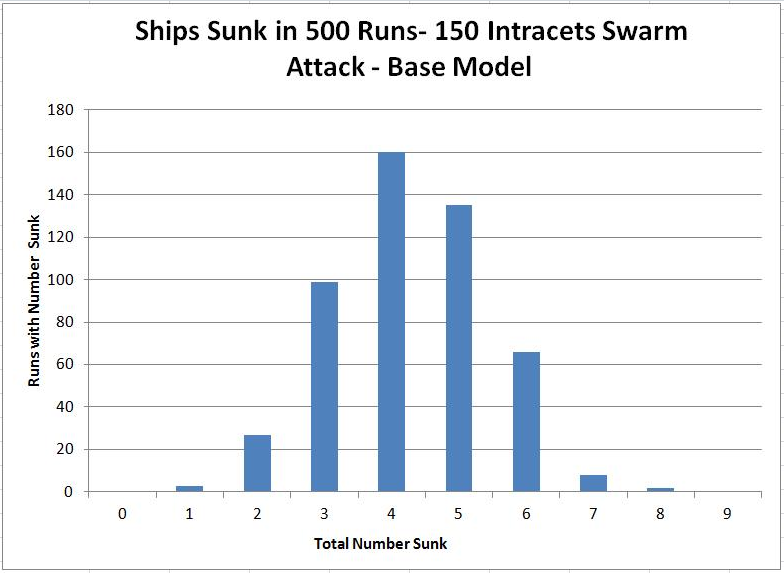
\includegraphics[scale=0.4]{images/ShipsSunk500Runs.png}
	\end{center}
	\caption{Ships sunk based on 500 runs of our model.}
	\label{fig:shipsSunk500Runs}
\end{figure}
\end{samepage}

\section{Base Model Adjustments}

\subsection{Cost Effective Improvements}
% Requirement 6
After conducting a study of potential capability insertions and upgrades to the given force package, a cost effective set of improvements to ensure less than 1\% chance of losing an ExWar ship in the scenario provided consists of a) adding 1 destroyer to the formation, b) increasing the probability of kill for the standard-2 missiles to 0.85 from the present 0.7 when intercepting Intracet threats, and c) increasing the threat detection range to 36,000 yards from the present 24,000 yards. This would reduce the probability of an ExWar sink occurring to 0.006 with 90\% confidence interval limits of 0.0117 and 0.0003.

The following represents the order of effectiveness of the factors based on the results of our design of experiment calculations.
\begin{enumerate}
	\item Detection range 
	\item Number of Destroyers 
	\item Probability of kill, $p(k)$, of the Standard-2 missile
	\item Interaction of detection range and number of destroyers 
	\item Interaction of detection range and probability of kill, $p(k)$, of the Standard-2 missile
	\item Interaction of probability of kill, $p(k)$ of the Standard-2 missile and the number of destroyers 
\end{enumerate}

And just below the cutoff for significance was the interaction of detection range and $p(k)$ of the CIWS.

The back of the envelope model was iterated with a variety of upgrades to study the effects of the potential upgrade improvements to improve survivability of the formation with the baseline case salvo (see Table \ref{tab:improvements} on page \pageref{tab:improvements}).  Other improvements analyzed include adding a cruiser to the formation, increasing the performance of the detection and classification element, adding missiles to the cruiser and destroyer platforms, and improving the probability of kill for the Close In Weapons System (CIWS).

Numerous sources were researched for developing cost estimates.  Among the sources investigated were publicly available market research including Missile Defense Agency information, the NASA cost estimating site for hardware, and the NAVY VAMOSC database.

\begin{figure}[h!tbp]
	\begin{center}
		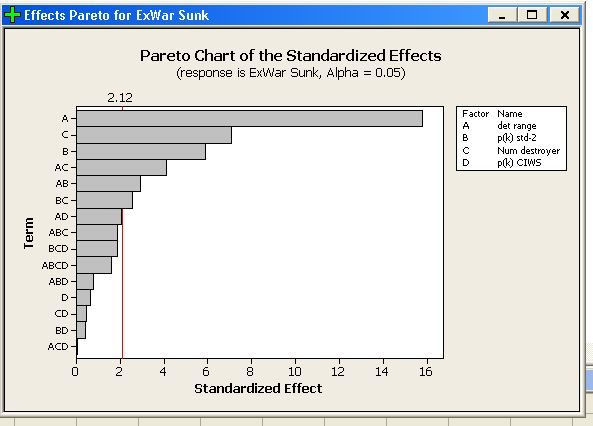
\includegraphics[scale=0.75]{images/Pareto.JPG}
	\end{center}
	\caption{Ordered list of prioritized factors for 2-level full-factorial.}
	\label{fig:pareto}
\end{figure}

The back of the envelope iterations were surveyed with a sort of a trial and error observation process to select a downsized set of parameters to study in a statistical analysis package to conduct a design of experiments to determine the most important factors influencing the result of number of ExWar ships sunk. The four factors and their interactions that were chosen for study were Detection Range, Number of Destroyers, probability of kill for Standard-2 missile, and probability of kill for Close In Weapons Systems. Two levels were established for the full factorial design. The low levels consisted of the existing system capabilities; 24,000 yards, 3, 0.70, and 0.30 respectively. The high levels represented 50\% improvements in three of the capabilities and an increment of one destroyer; 36,000 yards detection range, $p(k)$ of 0.85 for Standard-2 missile, and $p(k)$ of 0.45 for Close In Weapons Systems. The results showed that all individual factors were significant with the exception of Close In Weapons System $p(k)$. This could be due to the modeling assumptions of the limited range of effectiveness and the amount of time for the CIWS to acquire the subsequent target. The adjusted $R^{2}$ for this full factorial was 92.2\%. This could be due to the decision made to not bring all of the factors iterated in the back of the envelope model into the statistical analysis package.

\begin{table}[h!tbp]\small
	\begin{center}
		\begin{tabular}{lc.}
			\hline
			\myalign{p{1.5cm}}{\textbf{Improvement}}
				& \myalign{p{1.5cm}}{\textbf{Cost}}
				& \myalign{p{2.2cm}}{\textbf{ExWars Sunk}}  \\
			\hline\hline
			Detect sense + p(k) std ��� 2 + Destroyer & \$1,293.30M & 0.002 \\
			Detect sense + Destroyer + CIWS & \$1,298.88M & 0.806 \\
			Detect sense + p(k) std ��� 2 + Cruiser & \$3,393.20M & 0 \\
			Detect sense + Cruiser + CIWS & \$3,398.88M & 0.82 \\
			Detect sense + Cruiser + Destroyer & \$4,491.08M & 0.068 \\
			\hline
		\end{tabular}
	\end{center}
	\caption{Acceptable model improvements ranked by cost.}
	\label{tab:improvements}
\end{table}

\subsection{Adjustment to Fleet Size}
% Requirement 7
Another excursion applied to the back of the envelope model was to sequentially add destroyers to the formation until a less than 1\% chance of losing an ExWar ship had been achieved.  The remaining system parameters and capabilities were left unchanged.  With the addition of five destroyers to the formation, the goal is nearly achieved.  Six additional destroyers will drive down the expectation for an ExWar sinking under the baseline salvo of 150 simultaneously fired Intracets down to 0.238.  90\% confidence interval limits are 0.277 and 0.199 based on 500 iterations of the back of the envelope model.  The team chose to add destroyers as opposed to cruisers due to the reduced acquisition costs associated with the former.  The base case scenario with the missile detection range set at its current distance capability does not permit leveraging the extra standard-2 missiles that a cruiser carries, compared to a destroyer, before the threats have passed inside the minimum engagement range.  Using this assumption, the costs associated with the six additional destroyers are 6.6 billion.  This is not cost-efficient compared to the recommended system upgrades of adding one destroyer, increasing the threat detection range, and raising the probability of kill for the standard-2 missiles when intercepting the Intracet threats.

\begin{table}[h!tbp]\scriptsize
	\begin{center}
		\begin{tabular}{lccc..}
			\hline
			& \myalign{c}{\textbf{Baseline}} 
				& \myalign{c}{\textbf{50\% Improvement}} 
				& \myalign{c}{\textbf{Cost}} 
				& \myalign{c}{\textbf{Total Sunk}}
				& \myalign{c}{\textbf{ExWars Sunk}}  \\
			\hline\hline
			\textbf{baseline} & - & - & - & 4.844 & 3.35 \\
			\textbf{+ 6 Destroyers} & Baseline = 3 & +6 & \$6.6 billion & 0.3 & 0.238 \\
			\hline
		\end{tabular}
	\end{center}
	\caption{Effects of adding 6 Destroyers.}
	\label{tab:R7a}
\end{table}

%Requirement 8
Figure \ref{fig:ce} on page \pageref{fig:ce} shows the results of our cost-effectiveness analysis for fleet protection improvement.  What it shows supports our recommendation to increase missile detection range, increase probability of intercept, and add one Destroyer.

\begin{figure}[h!tbp]
	\begin{center}
		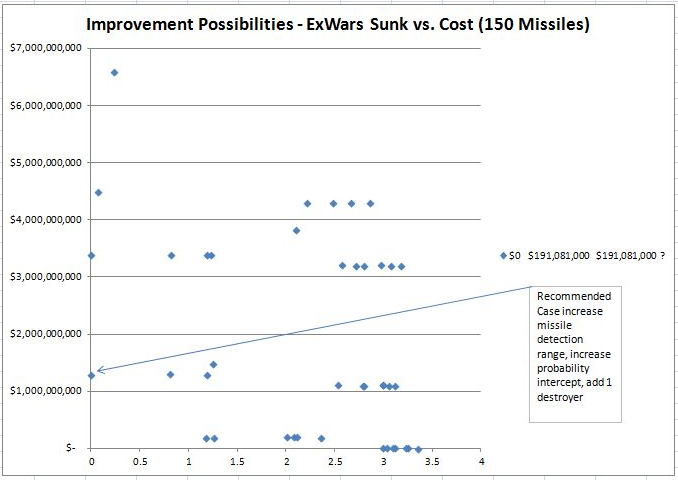
\includegraphics[scale=0.6]{images/costEffectiveness.png}
	\end{center}
	\caption{Improvement possibilities: ExWars sunk vs. cost.}
	\label{fig:ce}
\end{figure}

\subsection{Adjustment to Incoming Salvo}
% Requirement 9
The back of the envelope model was modified to change the size of the salvo threatening the existing force package.  The first change lowered the number of missiles to 50 in the salvo, and the second change raised the number of missiles in the salvo to 200.  No other parameters were modified besides number of incoming Intracets.

The 50 missile case was demonstrated to be no threat to the formation.  Across the 500 runs, there was not a single instance of enough leaker missiles passing inside the minimum standard-2 engagement range to overcome the 9 ships' Close In Weapons Systems to neutralize the threat.

The 200 missile case showed the other end of the scenario space.  The threat that the group faces in the base case is magnified with the addition of one third more incoming Intracets.  The mean number of ExWars sunk raises to 3.77 average over the 500 runs.  The Super Leaker quantities range from a minimum of 115 to 145 maximum, which is nearly the size of the baseline case salvo (150).  This contributes to increasing the average number of ships sunk to 6.04, two thirds the size of the group.  Nearly 1.5 destroyers are predicted to sink, and almost 1.0 cruiser.  There are over 103 expected super leaker strikes on ships, distributed according to radar cross sections in the model.  That allocation is over 20 strikes per ExWar ship and at least one on each of the 5 destroyers or cruisers in the group.

\subsection{Adjustment for Simultaneous Arrival}
% Requirement 10a
The ExtendSim model was adjusted to allow the Intracets to not be fired simultaneously, but with an expected arrival time with a standard deviation of 30 seconds.  It was our expectation that this change would spread out the arrival time and allow the cruisers and destroyers more time to fire S2 missiles, which would intercept more Intracets and reduce the attack damage to the ship force substantially.  However, the metric results based on 500 model runs (See Tables \ref{tab:10a1} - \ref{tab:10a3} beginning on page \pageref{tab:10a1}) indicate that not much has changed when compared to base model results.  The results indicate an average of 4.37 ships are sunk per run and 64.18 Intracets killed by S2 missiles.

\begin{table}[h!tbp]\small
	\begin{center}
		\begin{tabular}{rcccc}
			\hline
			& \textbf{ExWars Sunk} & \textbf{Cruisers Sunk} & \textbf{Destroyers Sunk} & \textbf{Total Sunk}  \\
			\hline\hline
			\textbf{Average} & 3.282 & 0.49 & 0.594 & 4.366 \\
			\textbf{Best} & 1 & 0 & 0 & 1 \\
			\textbf{Worst} & 4 & 2 & 3 & 8 \\
			\hline
		\end{tabular}
	\end{center}
	\caption{Ships sunk with simultaneous arrival time.}
	\label{tab:10a1}
\end{table}

\begin{table}[h!tbp]\small
	\begin{center}
		\begin{tabular}{rcccccc}
			\hline
			& \myalign{p{1.5cm}}{\textbf{ExWars Hit}}
				& \myalign{p{1.5cm}}{\textbf{Cruisers Hit}}
				& \myalign{p{2.2cm}}{\textbf{Destroyers Hit}}
				& \myalign{p{1.5cm}}{\textbf{ExWars Missed}}
				& \myalign{p{1.5cm}}{\textbf{Cruisers Missed}}
				& \myalign{p{2.2cm}}{\textbf{Destroyers Missed}}  \\
			\hline\hline
			\textbf{Average} & 49.43 & 1.81 & 1.03 & 14.12 & 0.53 & 0.40 \\
			\textbf{Best} & 36 & 0 & 0 & 5 & 0 & 0 \\
			\textbf{Worst} & 65 & 7 & 6 & 27 & 4 & 4 \\
			\hline
		\end{tabular}
	\end{center}
	\caption{Missile hits and misses by ship platform.}
	\label{tab:10a2}
\end{table}

\begin{table}[h!tbp]\small
	\begin{center}
		\begin{tabular}{rccccc}
			\hline
			& \textbf{S2} & 
				\textbf{ExWar CIWS} & 
				\textbf{Cruiser CIWS} & 
				\textbf{Destroyer CIWS} & 
				 \textbf{Total CIWS}  \\
			\hline\hline
			\textbf{Average} & 64.176 & 8.35 & 1.27 & 0.79 & 10.41 \\
			\textbf{Best} & 75 & 17 & 6 & 5 & 20 \\
			\textbf{Worst} & 47 & 1 & 0 & 0 & 2 \\
			\hline
		\end{tabular}
	\end{center}
	\caption{Missile kills with simultaneous arrival time.}
	\label{tab:10a3}
\end{table}

\subsection{Adjustment for Selective Initial Targeting}
% Requirement 10b
The ExtendSim base model was adjusted to allow the first 25\% (or 38) of the Intracets to only target the cruisers and the destroyers.  The remainder of the Intracets in the attack target ships according to ship RCS.  It was assumed any cruisers and destroyers sunk in the Intracet attack retain a fighting capability throughout the attack and sink sometime after the attack has been completed.  This allows the cruisers and destroyers to use their S2 missiles and CIWS during the attack.    The attack results in an average number of ships sunk of 5.936.  As expected, the focused attack is more effective in sinking destroyers and cruisers.  This leaves the ship force highly susceptible to any additional attacks or if more than 150 Intracets are used by the enemy.   A column chart was constructed (see Figure \ref{fig:10b} on page \pageref{fig:10b}) and shows that in over 70\% of the simulation runs, 5 to 7 ships are sunk.


\begin{figure}[h!tbp]
	\begin{center}
		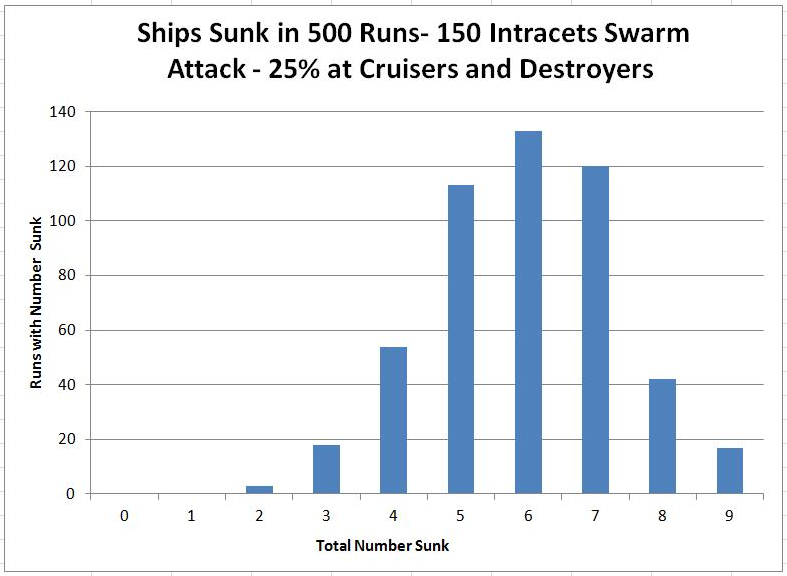
\includegraphics[scale=0.5]{images/10b.png}
	\end{center}
	\caption{Ships Sunk with 25\% of Intracets Attacking Cruisers and Destroyers.}
	\label{fig:10b}
\end{figure}

Data on the metrics of interest was collected (see Tables \ref{tab:10b1} - \ref{tab:10b3} beginning on page \pageref{tab:10b1}).  On average, the attack sinks more than 3 cruisers and destroyers per run, as opposed to 1 in the base model.  The ExWars were targeted less than when radar cross section (RCS) was the determining factor, but lose protection once cruisers and destroyers sink.

\begin{table}[h!tbp]\small
	\begin{center}
		\begin{tabular}{rcccc}
			\hline
			& \textbf{ExWars Sunk} & \textbf{Cruisers Sunk} & \textbf{Destroyers Sunk} & \textbf{Total Sunk}  \\
			\hline\hline
			\textbf{Average} & 2.862 & 1.058 & 2.016 & 5.936 \\
			\textbf{Best} & 1 & 0 & 0 & 2 \\
			\textbf{Worst} & 4 & 2 & 3 & 9 \\
			\hline
		\end{tabular}
	\end{center}
	\caption{Ships sunk with 25\% Targeting Cruisers and Destroyers.}
	\label{tab:10b1}
\end{table}

\begin{table}[h!tbp]\small
	\begin{center}
		\begin{tabular}{rcccccc}
			\hline
			& \myalign{p{1.5cm}}{\textbf{ExWars Hit}}
				& \myalign{p{1.5cm}}{\textbf{Cruisers Hit}}
				& \myalign{p{2.2cm}}{\textbf{Destroyers Hit}}
				& \myalign{p{1.5cm}}{\textbf{ExWars Missed}}
				& \myalign{p{1.5cm}}{\textbf{Cruisers Missed}}
				& \myalign{p{2.2cm}}{\textbf{Destroyers Missed}}  \\
			\hline\hline
			\textbf{Average} & 35.47 & 5.13 & 5.04 & 10.20 & 1.54 & 2.12 \\
			\textbf{Best} & 22 & 1 & 0 & 3 & 0 & 0 \\
			\textbf{Worst} & 51 & 12 & 13 & 20 & 6 & 6 \\
			\hline
		\end{tabular}
	\end{center}
	\caption{Missile hits and misses by ship platform.}
	\label{tab:10b2}
\end{table}

\begin{table}[h!tbp]\small
	\begin{center}
		\begin{tabular}{rccccc}
			\hline
			& \textbf{S2} & 
				\textbf{ExWar CIWS} & 
				\textbf{Cruiser CIWS} & 
				\textbf{Destroyer CIWS} & 
				 \textbf{Total CIWS}  \\
			\hline\hline
			\textbf{Average} & 64.518 & 8.44 & 3.15 & 4.39 & 15.97 \\
			\textbf{Best} & 78 & 17 & 8 & 11 & 28 \\
			\textbf{Worst} & 49 & 2 & 0 & 0 & 7 \\
			\hline
		\end{tabular}
	\end{center}
	\caption{Missile kills with 25\% Targeting Cruisers and Destroyers.}
	\label{tab:10b3}
\end{table}

The results indicate how important it is to have a minimized radar cross section (RCS).  RCS is related to the geometry of the ships, the reflectivity or amount of power reflected back to the radar, and the directivity or the direction of the power reflected back to the radar.  Ability to the enemy to target the fighting ships within the force needs to be minimized in order to ensure effective protection of the ExWars.

\section{Summary}
What we find is that the System Design is incapable of sustaining attack in the scenario proposed without the loss of at least 1 high value target, even in the best cases.  Reducing this risk to within a 90\% confidence of a less than a 1\% chance of losing an ExWar ship from a salvo of 150 Intracets fired requires at least three improvements to the fleet at an estimated cost of about \$1.3 billion.
The improvements necessary include an increase in detect range,  an increase in the probability of kill, and the addition of one Destroyer.

\pagebreak
\appendix
\section{Range-Target Graph}

\begin{figure}[h!tbp]
	\begin{center}
		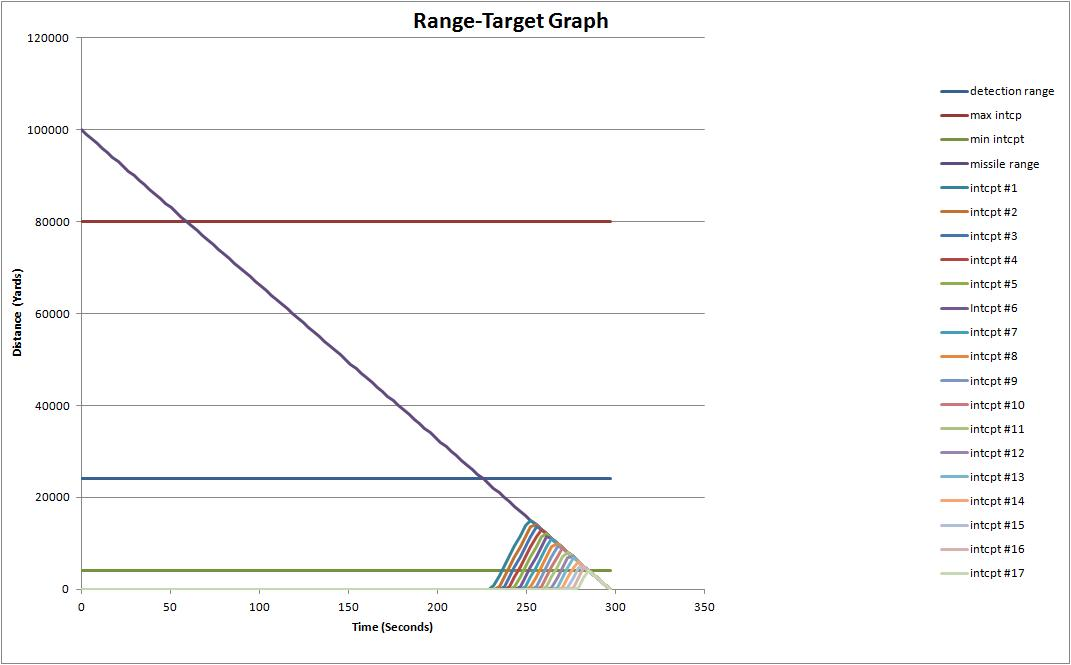
\includegraphics[scale=0.5]{images/Range-Target.jpg}
	\end{center}
	\caption{Range-target graph.}
	\label{fig:rangeTarget}
\end{figure}

\end{document}